\documentclass[t, notes, xcolor=table]{beamer}

\usepackage{wrapfig}
\usepackage{float}
% For tabs in verbatim
\usepackage{fancyvrb}

% Adjust position of the image
\usepackage[export]{adjustbox}

% set fonts
\usefonttheme{professionalfonts} % using non standard fonts for beamer
\usepackage{txfonts,mathptmx}

% set indend spacing for first and second level indentation
\setlength{\leftmargini}{0.5cm}
\setlength{\leftmarginii}{0.5cm}
\setlength{\leftmarginiii}{0.5cm}

% Set circles for bullets 
\setbeamertemplate{itemize items}[circle]

% colors
\usepackage{xcolor}

% multiple columns
\usepackage{multicol}

% todo lists
\usepackage{pifont}
\usepackage{amssymb}

% increase space between text and frame name
\addtobeamertemplate{frametitle}{}{\vspace{0.5em}}

%Information to be included in the title page:
\title{Directing the Compiler}
\author{Nikola Petrovic}
\institute{University of Belgrade, School of Electrical Engineering}
\date{2022}



\begin{document}

\frame{\titlepage}

%%%%%%%%%%%%%%%%%%%%%%%%%%%%%%%%%%%%%%%%%%%%%%%%%%%%%%%%%%%%
\begin{frame}
\frametitle{Module Objective}
In this module we will direct the compiler to interpret subsequent source code.
\newline

\textbf{Topics:}
\begin{itemize}
\item Substituting text
\item Conditionally compiling code
\item Including files
\item Setting the timescale
\item Reserving keywords
\item Using pragmas
\end{itemize}


\end{frame}
\note{
\scriptsize{
Out objective is to appropriately and effectively utilize compiler directives. To do that, we need to know what directives are available and what they do and how to use them.
\newline

 A compiler directive is a directive to the compiler. it is not syntactically a Verilog declaration or a Verilog statement. The scope of a compiler directive is from the point in the source stream input to the compiler to the point at which the directive is  or disabled ar the end of the compilation session, probably across multiple files and multiple module descriptions, and sometimes affecting only parts of files or parts of module descriptions.
 \newline
 
Verilog compiler directives are prefixed with the "back-tick" (`) character more formally called the \textbf{accent grave}. Wherever we see that character in Verilog code it is always associated with a compiler directive.
\newline

This module introduces compiler directives.  they are more closely related to lexical structure that to declaration and statements, we will understand them better if we have an understanding of Verilog declarations and statements. The course will later revisit many of these directives in an appropriate context that uses them 


}
}

%%%%%%%%%%%%%%%%%%%%%%%%%%%%%%%%%%%%%%%%%%%%%%%%%%%%%%%%%%%%
\begin{frame}[fragile]
\frametitle{Substituting Text: The `define Directive}
\scriptsize{
\begin{multicols}{2}
Define a text substitution macro:
\begin{Verbatim}[commandchars=\\\{\}, tabsize=2]
\textcolor{purple}{	\textbf{`define} name[(arguments)] text}
\end{Verbatim}
\begin{itemize}
\item Text can use other text macros.
\end{itemize}

\vspace{10pt}
Use a text substitution macro:
\begin{Verbatim}[commandchars=\\\{\}, tabsize=2]
\textcolor{purple}{	\textbf{`name}[(arguments)]}
\end{Verbatim}
\begin{itemize}
\item Preprocessor substitutes text literally (WYSIWYG).
\end{itemize}

\vspace{10pt}
Undefine a text macro:
\begin{Verbatim}[commandchars=\\\{\}, tabsize=2]
\textcolor{purple}{	\textbf{`undef} name}
\end{Verbatim}
\vfill
\columnbreak
\begin{figure}
    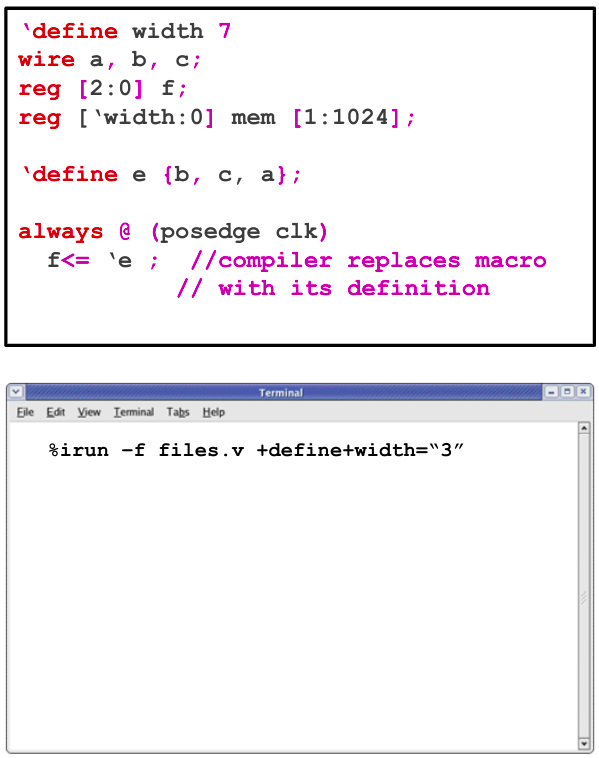
\includegraphics[width=0.45\textwidth]{img/11_define.png}
\end{figure}
\end{multicols}
}
\end{frame}
\note{
\tiny{
We can use the text substitution facility anywhere that we want to write generic code that we can then easily replace during subsequent compilation sessions without the need to edit the target source file. We can define the text substitution macros in a separate file that we compile first during the compilation session, and many tools also provide a vendor-dependent command-line way to define text substitution macros.
\newline

As the scope of a compiler directive depends upon compilation order and thus can change between compilation sessions, we may want to instead use module parameters wherever possible for design constants such as delays and vector widths.
\newline

We can place a \textit{`define} directive anywhere in our source code, but most people by convention place them all in a separate file, or at the top of the file if they are used in only one file.
\begin{itemize}
\item Text macros have their own name space. We can define a macro with the same name as a module without causing confusion. We cannot name the text macro with the same name as an existing compiler directive, as that would definitely cause confusion.
\item We can include a parenthesized list of formal arguments, The opening parenthesis must appear immediately after the macro identifier with no intervening white space.
\item A newline character terminates the macro definition. We can escape the newline with a backslash (\textbackslash) character to continue the definition on a subsequent line.
\item Some constructs we cannot split across text macros. This means that if a macro definition starts the construct then it must complete the construct in that same macro definition. Constructs we cannot split across text macros are comments, identifiers, keywords, numbers, operators and strings.
\end{itemize}

}
}

%%%%%%%%%%%%%%%%%%%%%%%%%%%%%%%%%%%%%%%%%%%%%%%%%%%%%%%%%%%%
\begin{frame}
\frametitle{Conditionally Compiling Code: The `ifdef Directive}

\begin{multicols}{2}

\footnotesize{
Conditionally compile code regions:
}
\scriptsize{
\begin{itemize}
\item Verilog 1995: \textbf{`ifdef, `else, `endif}
\item Verilog 2001: \textbf{`ifndef, `elsif}
\item We can define the macros without providing a value
\item Many tools provide a vendor-dependant command-line way to set text replacement macros
\end{itemize}
\vfill
\columnbreak
\begin{figure}
    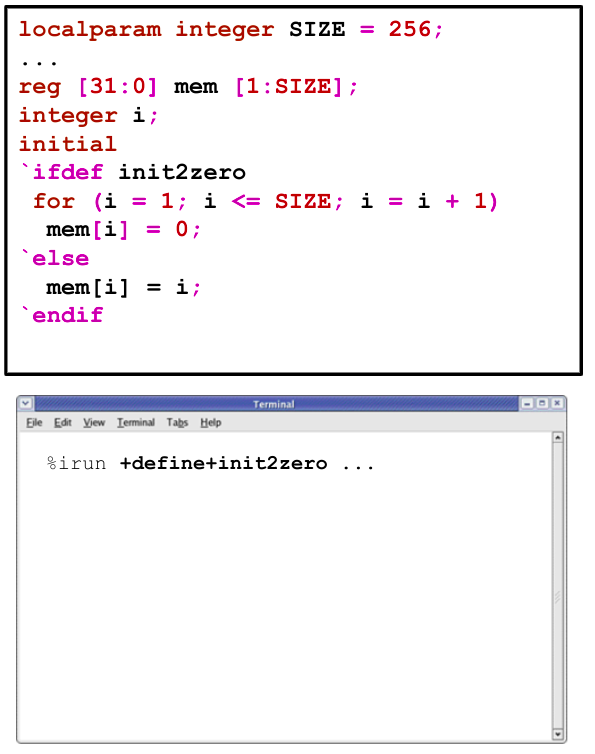
\includegraphics[width=0.45\textwidth]{img/11_ifdef.png}
\end{figure}
}
\end{multicols}

\end{frame}
\note{
\scriptsize{
We can use the existence of a text macro to conditionally compile lines of source code.
\newline

We use these directives similarly in an algorithmic sense to the \textit{if-else} statement, but of course keep in mind that these macros must each appear on their own line and it is the preprocessor that parses them during compile time.
\newline

This example provides the option to initialize the ROM to either all zeros or to values read from a file.

}
}

%%%%%%%%%%%%%%%%%%%%%%%%%%%%%%%%%%%%%%%%%%%%%%%%%%%%%%%%%%%%
\begin{frame}[fragile]
\frametitle{Including Files: The `include Directive}
\scriptsize{
\begin{multicols}{2}
Insert the contents of a source file:
\begin{Verbatim}[commandchars=\\\{\}, tabsize=2]
\textcolor{purple}{	\textbf{`include} "\textit{filename}"}
\end{Verbatim}
\begin{itemize}
\item Use included files to ensure that team-wide module descriptions use the same declarations:
\begin{itemize}
	\scriptsize{
	\item Constants
	\item Functions and tasks	
	}
\end{itemize}
\item The included file can contain another `include directive:
\begin{itemize}
	\scriptsize{
	\item The standard guarantees nesting up to 15 deep	
	}
\end{itemize}
\end{itemize}
\vfill
\textcolor{purple}{*The double-quoted argument is a literal string so cannot be a text macro.}
\columnbreak
\begin{figure}
    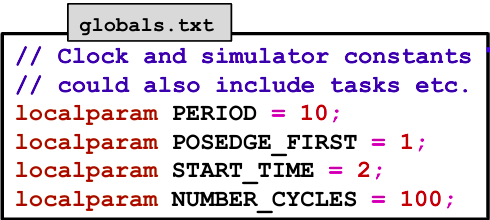
\includegraphics[width=0.45\textwidth]{img/11_include1.png}
\end{figure}
\begin{figure}
    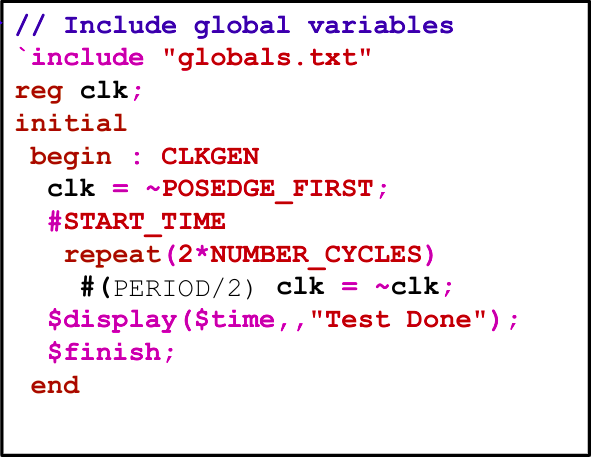
\includegraphics[width=0.45\textwidth]{img/11_include2.png}
\end{figure}
\end{multicols}
}

\end{frame}
\note{
\scriptsize{
The \textit{`include} directive includes the contents of a file at the point where the directive appears. The effect is exactly as if the file contents were copied into the source at that point to replace the \textit{`include} directive.
\newline

People use this directive to include declarations that are used by all team members and so for the sake of consistency should be maintained in one place.
\newline

The standard guarantees that we can nest included files at least 15 deep.
\newline

The argument to the \textit{`include} directive is a quoted file path name and not a compiler directive or string literal. No standard way exists to generate the file name to be included.

}
}

%%%%%%%%%%%%%%%%%%%%%%%%%%%%%%%%%%%%%%%%%%%%%%%%%%%%%%%%%%%%
\begin{frame}[fragile]
\frametitle{Setting the Timescale: The `timescale Directive}
\scriptsize{
\begin{multicols}{2}
Set time unit and time precision:
\begin{Verbatim}[commandchars=\\\{\}, tabsize=2]
\textcolor{purple}{	\textbf{`timescale} \textit{unit}\textbf{/}\textit{precision}}
\end{Verbatim}
\begin{itemize}
\item 1 or 10 or 100 followed by unit.
\item \textit{unit} can be \verb+fs, ps, ns, us, ms, s+.
\item \textit{precision} cannot be larger than unit.
\item The simulator rounds time specifications to the precision of the module and scales them to the time unit of the module.
\item The overall simulation precision is the smallest of the defined precisions.
\item \textbf{`timescale} must appear outside of the module!
\end{itemize}
\vfill
\columnbreak
\begin{figure}
    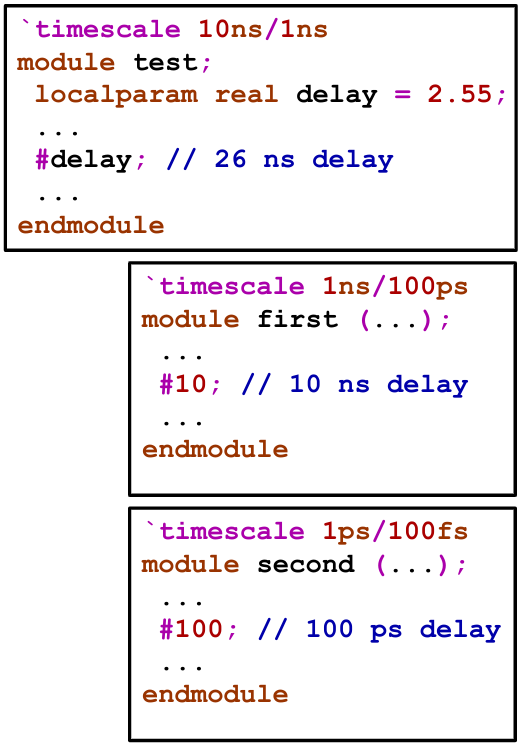
\includegraphics[width=0.45\textwidth]{img/11_timescale.png}
\end{figure}
\end{multicols}
}
\end{frame}
\note{
\tiny{
The \textit{`timescale} directive specifies the time unit and time precision for subsequent module declarations. Any expression used in a context to mean simulation time will assume the time unit of the current module and be rounded to the time precision of the current module. System tasks that display simulation time will scale the display to the time unit of the current module.
\newline

As the standard does not prescribe a default time scale, for interoperability either all modules must be subject to a time scale or no module can be subject to a time scale. To ensure that all modules are subject to a time scale, we should get used to specifying the time scale at the top of every file, even if we must not use time specifications in the file. To modify a time scale, we need to edit the file and recompile that file and all other files that utilized that directive. No method exists to modify a time scale during simulation.
\newline

Cadence requires either all modules to have a time scale or we can instead of specifying a time scale at each module, we can instead give it as a command line option. The \textit{-timescale} option provides a default timescale for the gate-level description. For example: \textit{irun -timescale 1ns/10ps}.
\newline

In this example, the file containing the \textit{test} module specifies that until further notice all subsequent time specifications are in units of 10ns and the time precision is 1ns. The 2.55 real value when used as a delay then means 25.5ns and is rounded to 26ns. The file containing the "second" module specifies that until further notice all subsequent time specifications are in units of 1ps and the time precision is 100fs. As this is the finest precision that any of these modules uses, if no other module requires a finer precision, this is the precision of the simulation.

}
}

%%%%%%%%%%%%%%%%%%%%%%%%%%%%%%%%%%%%%%%%%%%%%%%%%%%%%%%%%%%%
\begin{frame}[fragile]
\frametitle{Reserving Keywords: `begin\_keywords, `end\_keywords}
\scriptsize{
\begin{multicols}{2}
Reserve keywords for identifiers:
\begin{Verbatim}[commandchars=\\\{\}, tabsize=2]
\textcolor{purple}{	\textbf{`begin_keywords}} "\textit{version_spec}"
\textcolor{purple}{	\textbf{`end_keywords}}
\end{Verbatim}

\begin{itemize}
\item Verilog-2005 directive for reserving keywords for user identifiers
\item Place outside design element
\begin{itemize}
\scriptsize{
	\item \textbf{config, module, primitive}
}
\end{itemize}
\item Version specifier:
\begin{itemize}
\scriptsize{
	\item 1364-1995
	\item 1364-2001-noconfig
	\item 1364-2001
	\item 1364-2005
}
\end{itemize}
\end{itemize}
\vfill
\columnbreak
\begin{figure}
    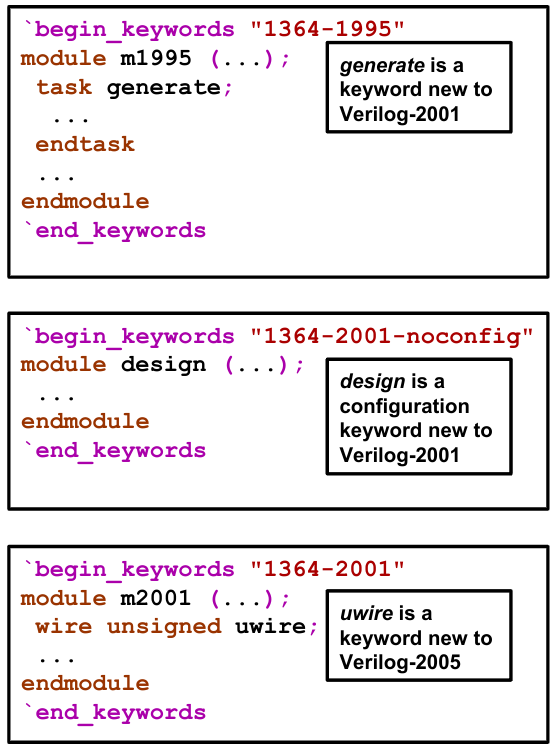
\includegraphics[width=0.45\textwidth]{img/11_reserve_keywords.png}
\end{figure}
\end{multicols}

}
\end{frame}
\note{
\tiny{
The \textit{`begin\_keywords} directive tells a parser to reserve for user identifiers all new keywords defined by a later standard. These keywords can appear only outside design elements, such as outside configuration, module, or primitive declarations.
\newline

If we have a legacy module that uses the \textit{generate} word as a user identifier, then we can direct a Verilog 2005 compliant compiler to not use nay keywords more recent than the 1995 standard for that module.
\newline

If we have a legacy module that uses the \textit{design} word as a user identifier, we can direct a Verilog 2005 compliant compiler to not use any Verilog 2001 configuration keywords or any other keywords more recent than the Verilog 2001 standard for that module.
\newline

If we have a legacy module that uses the \textit{uwire} word as a user identifier, we can direct a Verilog 2005 compliant compiler to not use any keywords more recent than the 2001 standard for that module.
\newline

\textbf{Keywords new to IEEE Std 1364-2001}: \textit{automatic, cell, config, design, endconfig, endgenerate, generate, genvar, incdir, include, instance, liblist, library, localparam, noshowcancelled, pulsestyle\_onevent, pulsestyle\_ondetect, showcancelled, signed, unsigned, use}
\newline

\textbf{Keywords new to IEEE Std 1364-2006}: \textit{uwire}
}
}

%%%%%%%%%%%%%%%%%%%%%%%%%%%%%%%%%%%%%%%%%%%%%%%%%%%%%%%%%%%%
\begin{frame}[fragile]
\frametitle{Using Pragmas: The `pragma Directive}
\scriptsize{
\begin{multicols}{2}
Utilize a pragma:
\begin{Verbatim}[commandchars=\\\{\}, tabsize=2]
\textcolor{purple}{	\textbf{`pragma}} \textit{pragma_name}
	[ \textit{pragma_expression} 
	\{, pragma_expression \} ]
\end{Verbatim}
\vspace{10pt}
\begin{itemize}
\item Verilog-2005 structure for implementation-specific directives
\vspace{10pt}
\item Verilog defines just a few:
\begin{itemize}
\scriptsize{
	\item \verb+`pragma reset+
	\item \verb+`pragma resetall+
	\item \verb+`pragma protect+
}
\end{itemize}
\end{itemize}
\vfill
\columnbreak
\begin{figure}
    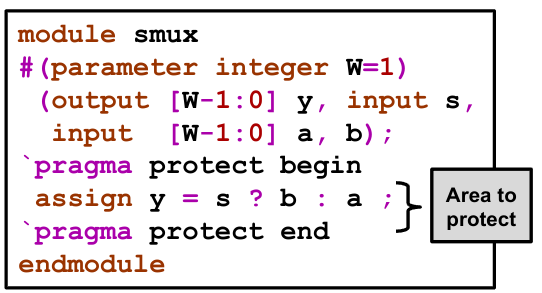
\includegraphics[width=0.45\textwidth]{img/11_pragma.png}
\end{figure}
\end{multicols}
}
\end{frame}
\note{
\tiny{
The \textit{`pragma} directive provides a means for implementations to extend the set of compiler directives. A pragma name follows the directive and is followed by an optional list of pragmas expressions. A pragma expression is a pragma keyword or a pragma value or an assignment of a pragma value to a pragma keyword.
\newline

The Verilog 2005 update defines only a few pragmas:
\begin{itemize}
\item The \textit{reset} pragma resets the pragmas provided as pragma expressions;
\item The \textit{resetall} pragma resets all pragmas;
\item The \textit{protect} pragma encrypts subsequent source code.
\end{itemize}
A implementation ignores pragmas it does not recognize.
\begin{figure}
    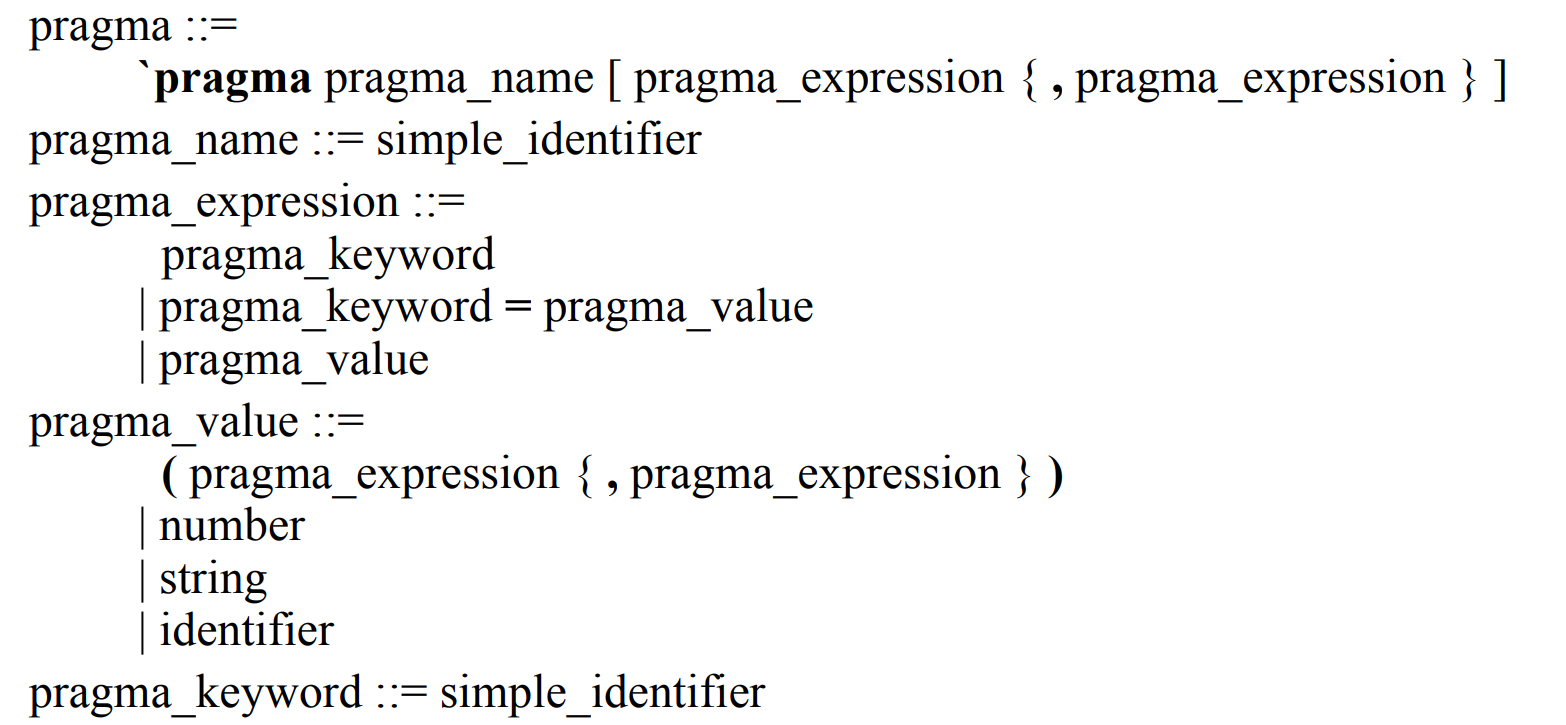
\includegraphics[width=0.65\textwidth]{img/11_pragma_syntax.png}
\end{figure}

}
}

%%%%%%%%%%%%%%%%%%%%%%%%%%%%%%%%%%%%%%%%%%%%%%%%%%%%%%%%%%%%
\begin{frame}[fragile]
\frametitle{Disable Implicit Net Declarations}
\begin{Verbatim}[commandchars=\\\{\}, tabsize=2]
\textcolor{purple}{\textbf{`default_nettype}}
\end{Verbatim}
New default net type: \textbf{none}
\normalsize{
\begin{itemize}
\item Verilog-1995 permits implicit net declarations.
\begin{itemize}
	\scriptsize{
	\item Use a previously undeclared identifier in a port expression or terminal list
	\item Becomes the default net type (initially a \textbf{wire})
	\item We change the default net type with \textbf{`default\_nettype}
	\begin{itemize}
		\scriptsize{
		\item \textbf{tri tri0 tri1 triand trior trireg wand wire wor}
		}
	\end{itemize}
	}
\end{itemize}
\item Verilog-2001 adds the default net type \textbf{none}
\begin{itemize}
	\scriptsize{
	\item Set this as the default net type with \textbf{`default\_nettype none}
	\item Undeclared signals become a syntax error
	\begin{itemize}
		\scriptsize{
		\item Reduces potential for typographical errors
		}
	\end{itemize}
	}
\end{itemize}
\end{itemize}
}
\end{frame}
\note{
\scriptsize{
We implicitly declare a net when we use a previously undeclared identifier in a port expression or terminal list or as the lvalue of a continuous assignment. That net by default becomes \textbf{wire}. We set the value of the \textit{`default\_nettype} directive to change that default net type. The Verilog 2001 standard adds the \textit{none} type. When we set the default net type to \textit{none}, we require explicit declaration of all nets, thus reducing the potential for typographical error.
\newline

\textbf{Note}: All Verilog compiler directives start with the grave accent (sometimes called a back-tick". We should be aware that some fonts cannot render this character properly and display it as an \textit{acute accent} (a "forward-tick").

}
}

%%%%%%%%%%%%%%%%%%%%%%%%%%%%%%%%%%%%%%%%%%%%%%%%%%%%%%%%%%%%
\begin{frame}
\frametitle{Reference: Compiler Directives}

\end{frame}
\note{

}

%%%%%%%%%%%%%%%%%%%%%%%%%%%%%%%%%%%%%%%%%%%%%%%%%%%%%%%%%%%%
\begin{frame}
\frametitle{Module}

\end{frame}
\note{

}

%%%%%%%%%%%%%%%%%%%%%%%%%%%%%%%%%%%%%%%%%%%%%%%%%%%%%%%%%%%%
\begin{frame}
\frametitle{Module}

\end{frame}
\note{

}

%%%%%%%%%%%%%%%%%%%%%%%%%%%%%%%%%%%%%%%%%%%%%%%%%%%%%%%%%%%%
\begin{frame}
\frametitle{Module}

\end{frame}
\note{

}

%%%%%%%%%%%%%%%%%%%%%%%%%%%%%%%%%%%%%%%%%%%%%%%%%%%%%%%%%%%%
\begin{frame}
\frametitle{Module}

\end{frame}
\note{

}

%%%%%%%%%%%%%%%%%%%%%%%%%%%%%%%%%%%%%%%%%%%%%%%%%%%%%%%%%%%%
\begin{frame}
\frametitle{Test You Understanding - 1}

\begin{itemize}
\item[$\square$] 
\item[$\square$] 
\item[$\square$] 
\item[$\square$] 
\end{itemize}
\end{frame}
\note{

}

\end{document}
